\documentclass{my-Presentation}
\usepackage{my-Pre-command}

% Title Page

\title[An FDM and PINN Comparison]{
  Meta-Programming and Hybrid Parallel Strategies for Solving PDEs: \\An FDM and PINN Comparison
  \footnote{full docs: \url{https://liyihai.com/html/index.html}}$^{,}$
  \footnote{repository: \url{https://github.com/liyihai-official/Final-Project}}
}
\subtitle{Seminar Presentation III}
\author[LI Yihai]{
  \normalsize
  LI YIHAI \\[1ex]
  \vspace*{-.5em}
}
\institute[Mathematics Institute]{
  Student ID: 23345919 \\[1ex]
  Supervision: Michael Peardon
}
\date{\today \vspace*{-1em}}
\titlegraphic{
\includegraphics[width=3cm]{logo.png}}


\begin{document}


\begin{frame}
  \titlepage
\end{frame}

\begin{frame}{Outline}
  \begin{multicols}{2}
    \tableofcontents
  \end{multicols}
\end{frame}

\section{Introduction}


\subsection{Related Work}
\begin{frame}
  \frametitle{Introduction}
  \framesubtitle{Recap - Deep Neural Network}
  \begin{block}{Kolmogorov PDEs}
    Solving $u(x,T)$, for 
    $\mathbb{R}^1\owns T>0$, 
    $x\in \mathbb{R}^d$, 
    $t\in [0,T]$,
    $\:u(t,x)=u \in \mathbb{R}^1$,
    $ \mu(x) \in \mathbb{R}^d$,
    $\sigma(x)\in \mathbb{R}^{d\times d}$,
    \begin{equation}
      u_t
      = \frac{1}{2}
      \Tr_{\mathbb{R}^d}\left[\sigma(x)\left[\sigma(x)\right]^*\Hess_x u\right] + 
      \left< \mu(x), \nabla_xu \right>_{\mathbb{R}^d}
    \end{equation}
  \end{block}
  \begin{figure}[htbp]
    \centering
      \begin{tikzpicture}[
        % Define styles
        neuron/.style={circle, draw, fill=blue!20, minimum size=1cm},
        arrow/.style={-Stealth},
        output/.style={circle, draw, fill=green!20, minimum size=1cm},
        scale=0.9,
        transform shape
    ]
        % Neuron
        \steporfull<1->{
          \node[] (input1) at (-1,-1.2) {$u(x,T)$};
        }

        \steporfull<1->{
          \node[] (neuron) at (-1,1) {$\mathbb{E} \left[\phi (X_{T}^{x})\right]$};
          \draw[arrow] (input1) -- (neuron) node[midway, above=0.5em, left=0.5em] {\itshape Feynman-Kac};
        }
        
        % \steporfull<1->{
          \node[right=5em of neuron] (input2) {
            $\displaystyle 
              \inf_{v \in C([a,b]^d,\mathbb{R})} 
              \mathbb{E}\left[ 
                \left| \phi(X_T^x) - v(\xi) \right|^2 
              \right]$
          }; % 使用 output 样式
          \draw[arrow] (neuron) -- (input2) node[midway, above=.5em] {\itshape Prop. 2.7};
        % }
        % % \itshape Discretization \& Th. 2.8
        % \steporfull<1->{
          % \draw[-{Latex[length=2mm,width=1.5mm]}] (input2.east) arc (0:70:6mm) node[midway, right] {};
          \draw[-{Latex[length=2mm,width=1.5mm]}] 
          ([xshift=6em]input2.south) 
          arc (-120:120:6mm) 
          node[midway, right] {\itshape Discretization \& Th. 2.8};
        % }

        % \steporfull<2->{
          
        % }
      
        % \steporfull<2->{
          \node[output, right=10em of input1] (output) {$\mathbb{U}(x; \theta)$};
          \node[right=5em of output] (input3) {Neural Network};
          \draw[arrow] (input3) -- (output) node[midway, below=.5em] {\itshape Prediction};
          \draw[arrow] (input2) -- (output) node[midway, right=.5em] {\itshape Loss Function};
        % }
        
        % \steporfull<2->{
          \draw[arrow] (output) -- (input1) node[midway, below=.5em] {\itshape $\approx$ to Solution};
        % }
    \end{tikzpicture}
    \caption{Deep Neural Network (DNN) Methodology of Solving Kolmogorov PDEs \cite{FIRST}}
    \label{<label>}
  \end{figure}
  

\end{frame}

\begin{frame}
  \frametitle{Introduction}
  \framesubtitle{Recap - Physics Informed Nerual Network}
  \begin{block}{General Form of PDEs}
    % \vspace{.5em}
    -- $u(t,x)$ denotes with the target function, $x\in \mathbb{R}^{d}$. \vspace{.5em}\\
    -- $\varGamma \left[\:\:\cdot\:\:; \lambda \right]$ is a non-linear operator parameterized by $\lambda$.
    \vspace{-.5em}
    \begin{equation}
      u_t(t,x) + \varGamma \left[u; \lambda \right] = 0
    \end{equation}
    \vspace{-1.5em}
      % \vspace*{1em}
      Define $f(t, x)$ to be given by 
      % \vspace*{1em}
      \begin{equation}
        f(t,x) = u_t(t,x) + \varGamma \left[u; \lambda \right]
      \end{equation}
      % \vspace*{.2em}
  \end{block}
  \begin{figure}[htbp]
    \centering
    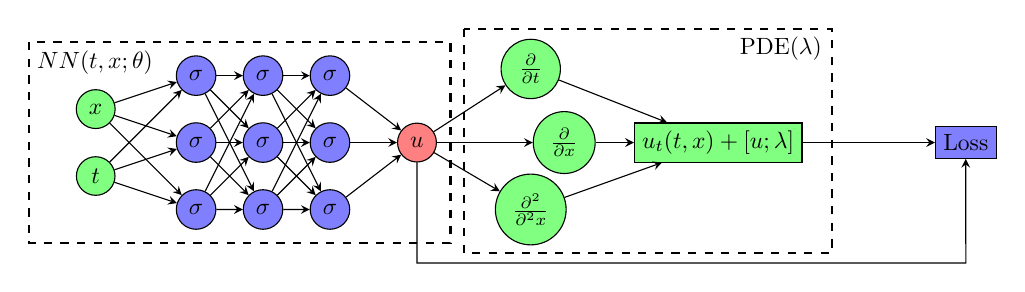
\begin{tikzpicture}[
      % Define styles
      neuron/.style={circle,draw,minimum size=.2cm},
      func/.style={rectangle,draw,minimum size=.2cm},
      PDE/.style={func, fill=green!50},
      loss/.style={func, fill=blue!50},
      input/.style={neuron, fill=green!50},
      hidden/.style={neuron, fill=blue!50},
      output/.style={neuron, fill=red!50},
      diff/.style={neuron, fill=green!50},
      arrow/.style={->,>=stealth},
      scale=0.85,
      transform shape
    ]
      
    \steporfull<3->{
      % Input Layer
      \draw[dashed, thick] (-1,0) rectangle (5.3,-3); % 前两个坐标为矩形左下角的坐标,后两个坐标为矩形右上角的坐标
      \node at (-1,0) [below right] {$NN(t,x; \theta)$}; % 文本内容为"文本",位置为方框的左上角

      \node[input] (Input0) at (0,-1) {$x$};
      \node[input] (Input) at (0,-2) {$t$};
    
      % Hidden Layer 1
      \node[hidden] (Hidden11) at (1.5,-0.5) {$\sigma$};
      \node[hidden] (Hidden12) at (1.5,-1.5) {$\sigma$};
      \node[hidden] (Hidden13) at (1.5,-2.5) {$\sigma$};
    
      % Hidden Layer 2
      \node[hidden] (Hidden21) at (2.5,-0.5) {$\sigma$};
      \node[hidden] (Hidden22) at (2.5,-1.5) {$\sigma$};
      \node[hidden] (Hidden23) at (2.5,-2.5) {$\sigma$};
    
      % Hidden Layer 3
      \node[hidden] (Hidden31) at (3.5,-0.5) {$\sigma$};
      \node[hidden] (Hidden32) at (3.5,-1.5) {$\sigma$};
      \node[hidden] (Hidden33) at (3.5,-2.5) {$\sigma$};

      % Output Layer
      \node[output] (Output) at (4.8,-1.5) {$u$};

      % Connect neurons Input-Hidden Layer 1
      \foreach \i in {1,2,3}
          \draw[arrow] (Input) -- (Hidden1\i);
        \foreach \i in {1,2,3}
          \draw[arrow] (Input0) -- (Hidden1\i);
    
      % Connect neurons Hidden Layer 1-Hidden Layer 2
      \foreach \i in {1,2,3}
          \foreach \j in {1,2,3}
              \draw[arrow] (Hidden1\i) -- (Hidden2\j);
    
      % Connect neurons Hidden Layer 2-Hidden Layer 3
      \foreach \i in {1,2,3}
          \foreach \j in {1,2,3}
              \draw[arrow] (Hidden2\i) -- (Hidden3\j);
    
      % Connect neurons Hidden Layer 3-Output
      \foreach \i in {1,2,3}
          \draw[arrow] (Hidden3\i) -- (Output);
    % }

    % \steporfull<2->{
      \draw[dashed, thick] (5.5,0.2) rectangle (11,-3.15);
      \node at (9.5,0.2) [below right] {PDE($\lambda$)}; % 文本内容为"文本",位置为方框的左上角
    %   % Partial Derivatives
      \node[diff] (D1) at (6.5,-0.4) {$\frac{\partial}{\partial t}$};
      \node[diff] (D2) at (7,-1.5) {$\frac{\partial}{\partial x}$};
      \node[diff] (D3) at (6.5,-2.5) {$\frac{\partial^2}{\partial^2 x}$};
      \node[PDE] (PDE) at (9.3,-1.5) {$u_t(t,x) + \varGamma \left[u; \lambda \right]$};

      \foreach \i in {1,2,3}
          \draw[arrow] (Output) -- (D\i);
      \foreach \i in {1,2,3}
          \draw[arrow] (D\i) -- (PDE);
    }

    % \steporfull<2->{
      \node[loss] (L) at (13,-1.5) {Loss};

      \draw[arrow] (Output) |- (13,-3.3) -- (L.south);
      \draw[arrow] (PDE.east) |- (L);
    % }
    \end{tikzpicture}
    \caption{PINN, with with 3 fully connected hidden layers}
    \label{}
\end{figure}
\end{frame}



\begin{frame}
  \frametitle{Introduction}
  \framesubtitle{Recap - Conclusion}
  \begin{block}{Comparing With Finite Difference Time Domain Method (FDTD)}
    \begin{enumerate}
      \item Deep Neural Network \cite{FIRST}
            \begin{itemize}
              \item Gives lower quality approximations.
              \item Takes longer time to train.
              \item Possible to solve high dimension PDEs \vspace*{1em}
            \end{itemize}
      \item Physics Informed Neural Network
            \begin{itemize}
              \item Gives higher quality approximations.
              \item Takes longer time to train.         
              \item Has more flexible way to get results.
              \item Possible to solve high dimension PDEs
            \end{itemize}
    \end{enumerate}    
  \end{block}
\end{frame}


% \subsection{Work Directions}
% \begin{frame}
%   \frametitle{Introduction}
%   \framesubtitle{Work Directions}
%   \begin{enumerate}
%     \item Implement FDTD and PINN in \texttt{C++/C}
%     \item Implement FDTD hybrid parallel version using \texttt{MPI/OpenMP}
%     \item Implement PINN GPU parallel version using \texttt{Libtorch/CUDA}
%     \item Performance optimization.
%     \item Running benchmarks
%   \end{enumerate}
% \end{frame}



\section{Problem Setups}

\subsection{General Form}
\begin{frame}
  \frametitle{General Form of problem}
  \begin{block}{}
    The PDE parametrized by number $\lambda$ and an operator $\mathcal{N}[\cdot; \lambda]$, 
    and assume the variable $x$ is a 2D or 3D spatio-vector which is written in 
    \begin{equation}
      \begin{cases}
        \displaystyle \frac{\partial u}{\partial t}\left(t,\vec{x}\right) + \mathcal{N}\left[u;\lambda\right] = 0 \\
        \displaystyle u\left(0,\vec{x}\right) = \varphi (\vec{x})
      \end{cases}
    \end{equation}
    where $\varphi$ is the initial condition, and $\vec{x}\in \Omega, t\in[0, +\infty)$.
  \end{block}


  \begin{block}{Boundary Conditions}
    The Dirichlet and Von Neurmann boundary conditions are formed as 
    \begin{equation}
      \begin{cases}
        \displaystyle u\left(t,\vec{x}\right) = g (t,\vec{x}) \\
        \displaystyle \frac{\partial u}{\partial \vec{n}} = g (t,\vec{x})  
      \end{cases}
    \end{equation}
    where $\vec{n}$ is the normal vector on $\overline{\Omega}$ the boundary of domain $\Omega$.
  \end{block}
\end{frame}


\subsection{Thermal Conduction Systems}
\begin{frame}
  \frametitle{Thermal Conduction Systems}
  \framesubtitle{Heat Equation 2D}
  \begin{block}{}
    The function 
    \begin{equation}
      u(t,x,y) = x + y - xy, \:\forall \alpha \in \mathbb{R}^1
    \end{equation}
    is the solution of 2D Heat Equation \ref{EQ:Heat2D} below
    \begin{align}\label{EQ:Heat2D}
      &\frac{\partial u}{\partial t} = \alpha \left(
        \frac{\partial u^2}{\partial^2 x}
        +
        \frac{\partial u^2}{\partial^2 y}
      \right) &(x,y) \in \Omega, \: t \in \left[0, +\infty\right)  \nonumber\\
      &u(0,x,y)  = \varphi(x,y) = 0 &(x,y) \in \Omega\\
      &u(t,x,y)
       = g(x,y)
       = \begin{cases}
        y, \:\: x=0, y\in\left(0,1\right)\\
        1, \:\: x=1, y\in\left(0,1\right)\\
        x, \:\: y=0, x\in\left(0,1\right)\\
        1, \:\: y =1, x\in\left(0,1\right)
      \end{cases}
      &t \in \left[0, +\infty\right) \nonumber
    \end{align}
  \end{block}
\end{frame}


\begin{frame}
  \frametitle{Thermal Conduction Systems}
  \framesubtitle{Heat Equation 3D}
  \vspace*{-0.3em}
  \begin{block}{}
    The function
    \begin{equation}
      u(t,x,y,z) = x + y + z - 2xy - 2xz - 2yz + 4xyz, \:\forall \alpha \in \mathbb{R}^1
    \end{equation}
    is the solution of 3D Heat Equation \ref{EQ:Heat3D} below
    \begin{align}\label{EQ:Heat3D}
      &\frac{\partial u}{\partial t} = \alpha \left(
        \frac{\partial u^2}{\partial^2 x}
        +
        \frac{\partial u^2}{\partial^2 y}
        +
        \frac{\partial u^2}{\partial^2 z}
      \right) & (x,y, z) \in \Omega, \: t \in \left[0, +\infty\right) 
                                                                      \nonumber\\
      &u(0,x,y,z)  = \varphi(x,y,z) = 0 &(x,y,z) \in \Omega\\
      &  u(t,x,y,z) = g(x,y,z) = 
      \begin{cases}
        y+z -2yz        , \:\: &x=0,\\
        1 - y - z + 2yz , \:\: &x=1,\\
        x+z - 2xz       , \:\: &y=0,\\
        1 - x - z + 2xz , \:\: &y =1,\\
        x+y - 2xy       , \:\: &z=0,\\
        1 - x - y + 2xy , \:\: &z=1
      \end{cases}
      &t \in \left[0, +\infty\right) \nonumber
    \end{align}
  \end{block}
\end{frame}

\section{Methodology}

\subsection{N-Dimension Matrix}
\begin{frame}
  \frametitle{N-dimension Matrix}
  \framesubtitle{STL containers}
  STL provides containers \texttt{std::array} and \texttt{std::vector} for creating one-dimension array.
  \\
  There are two way for dealing with high-dimension data:
  \begin{enumerate}
    \item Nesting the one dimension arrays or vectors.
    \item Hierarchy approach, designing derived classes of one-dimension array base class.
  \end{enumerate}
  \begin{figure}[htbp]
    \centering
    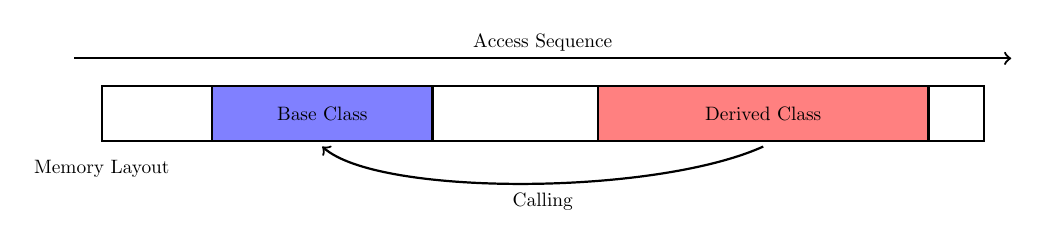
\begin{tikzpicture}[scale=0.7, transform shape]
      % \draw[help lines, step=1] (-10,-2) grid (10,2);    
      % % Draw axes
      % \draw[dashed,->] (-10,0) -- (10,0) node[right] {x};
      % \draw[dashed,->] (0,-2) -- (0,2) node[above] {y};

      \draw[thick, ->] (-8.5, 1.5) -- node[midway, above] {Access Sequence} (8.5, 1.5);

      \draw[thick] (-8,1) rectangle (8,0);
      \node at (-8,-0.5) [] {Memory Layout};

      \draw[thick, fill=blue!50] (-6,1) rectangle (-2,0);
      \node at (-4, 0.5) [] {Base Class};

      \draw[thick, fill=red!50] (1,1) rectangle (7,0);
      \node at (4, 0.5) [] {Derived Class};

      \node at (0, -1.1) [] {Calling};
      \draw[thick, ->] (4, -0.1) 
        .. controls (2, -1) and (-3, -1) .. (-4, -0.1);

    \end{tikzpicture}
    \caption{Derived Class calling members in Base class, timing is not predictable.}
    \label{<label>}
  \end{figure}
\end{frame}


\begin{frame}
  % \frametitle{N-dimension Matrix}
  % \framesubtitle{Memory Layout Problem}
  \begin{enumerate}
    \item Nesting multi-dimension array has non-contiguous memory layout.
    \item Derived class needs more time to access members in base class.
    \item Poor cache utilization leads to poor performance.
    \item MPI type create requires contiguous memory layout.
  \end{enumerate}
  % 插入图
  \begin{figure}[htbp]
    \centering
    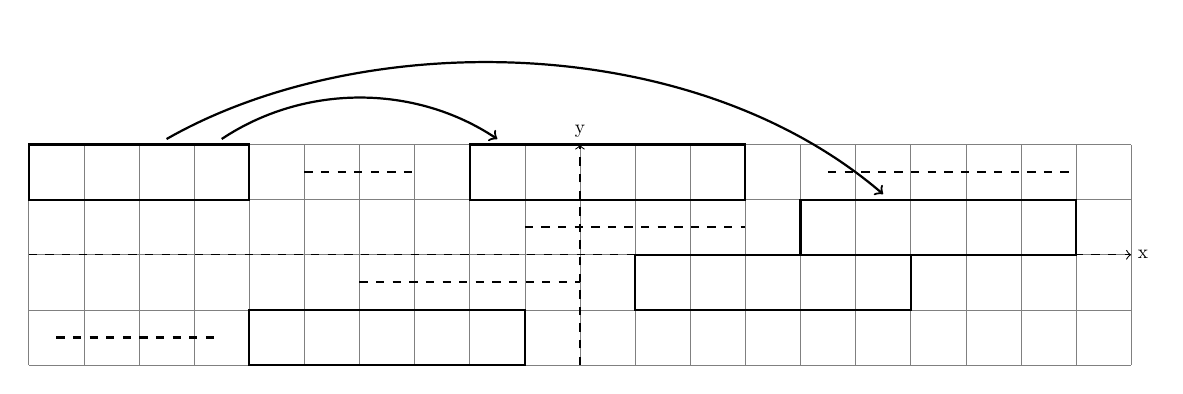
\begin{tikzpicture}[scale=0.7, transform shape]
      \draw[help lines, step=1] (-10,-2) grid (10,2);    
      % Draw axes
      \draw[dashed,->] (-10,0) -- (10,0) node[right] {x};
      \draw[dashed,->] (0,-2) -- (0,2) node[above] {y};

      \draw[thick] (-10,2) rectangle (-6,1);    
      \draw[dashed, thick] (-5,1.5) -- (-3, 1.5);

  
      \draw[thick] (-2,2) rectangle (3,1);
      \draw[dashed, thick] (4.5,1.5) -- (9, 1.5);

      \draw[dashed, thick] (-1,0.5) -- (3, 0.5);
      \draw[thick] (4,1) rectangle (9,0);
      

      \draw[thick] (1,0) rectangle (6,-1);
      \draw[dashed, thick] (-4, -0.5) -- (0, -0.5);

      \draw[dashed, thick] (-9.5, -1.5) -- (-6.5, -1.5);
      \draw[thick] (-6,-1) rectangle (-1,-2);


      \draw[thick, ->] (-6.5, 2.1) 
      .. controls (-5, 3.1) and (-3, 3.1) .. (-1.5, 2.1);

      \draw[thick, ->] (-7.5, 2.1) 
      .. controls (-4, 4.1) and (2, 4.1) .. (5.5, 1.1);
      
    \end{tikzpicture}
    \caption{<caption>}
    \label{<label>}
  \end{figure}
\end{frame}


\begin{frame}
  \frametitle{N-dimension Matrix}
  \framesubtitle{Solution}
  \begin{itemize}
    \item An external small \texttt{\_\_multi\_array\_shape} object defines the routines for accessing the elements.
    \item Smart pointer, ensure memory's contiguous layout and safety.
    \item Separate into two detail and user interface objects adhering RAII rules.
  \end{itemize}


  % 插入图
\end{frame}







\subsection{Parallelization of Multi-dimensional Matrices on cartesian Topologies}


% \section{Implementations}
% \subsection{PDE Solvers}
% % \subsection{General Setups}
% % \subsection{Parallel Strategies}


\subsection{PINN Model}


\section{Experiments}
\begin{frame}
  \frametitle{Hardware}

  \begin{block}{CPU cluster}
    Each node has a: \ttfamily{Intel(R) Xeon(R) Platinum 9242 CPU \@2.30Ghz, with 96 CPU(s)}
    \begin{table}
      \caption{Part outputs of \ttfamily{lscpu}}
      \begin{center}
        \footnotesize
        \begin{tabular}{p{1.5cm} p{1.5cm} p{1.5cm} p{1.5cm} p{1.5cm} p{1.5cm}} 
          \toprule
          \bfseries Attribute & \ttfamily{NUMA}& \ttfamily{L1d}      & \ttfamily{L1i}   & \ttfamily{L2} & \ttfamily{L3}      \\
          \midrule 
          \bfseries Values    & 4 & 32KB            & 32KB           &  1MB  &  35.75MB \\
          \bottomrule 
        \end{tabular}
      \end{center}
    \end{table}
  \end{block}

  \begin{block}{GPU cluster}
    Each node has a
    \begin{itemize}
      \item \ttfamily{AMD Ryzen 9700X3D, with 12 CPU(s)}
      \item \ttfamily{NVIDIA RTX 4090, 24GB}
    \end{itemize}
    
    
  \end{block}

\end{frame}

\subsection{On Single Node}
\begin{frame}
  \frametitle{Single Node Scaling Tests}
  2D Heat Equation\\
  Single Precision \\
  Problem Size: $512^2, 1024^2, 2048^2, 4096^2, 8192^2, 16384^2, 32768^2$ \\
  Non-unified Memory Access (NUMA) node Topology:
  \begin{figure}[htbp]
    \centering
    \begin{tikzpicture}[scale=0.6, transform shape]
      % \node[anchor=south west,inner sep=0] (image) at (0,0) {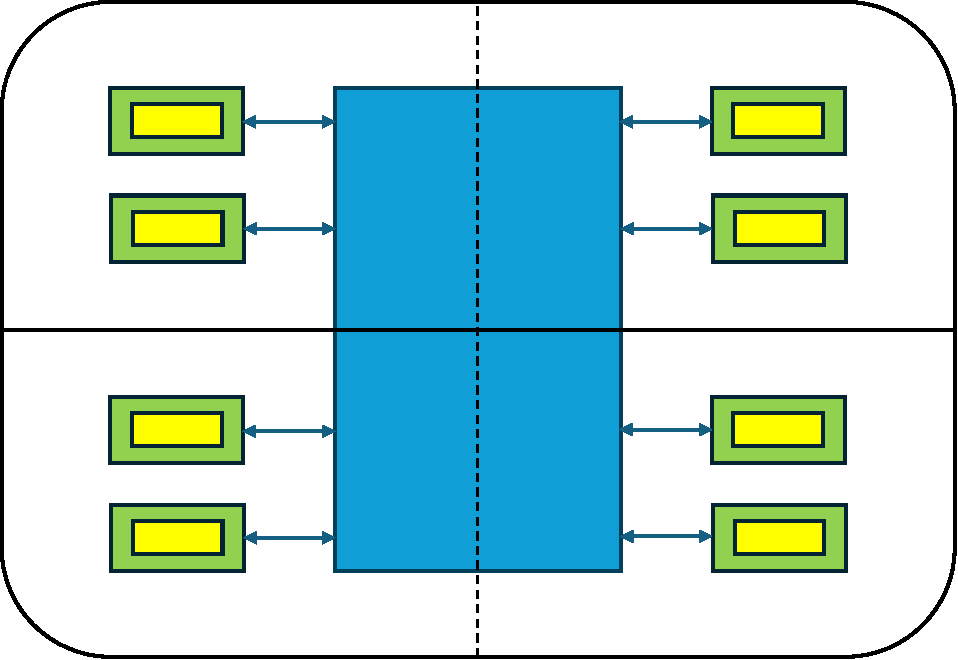
\includegraphics[width=0.5\textwidth]{figure/FIG_Topology_9242.pdf}};
      \node[anchor=south west,inner sep=0] (image) at (0,0) {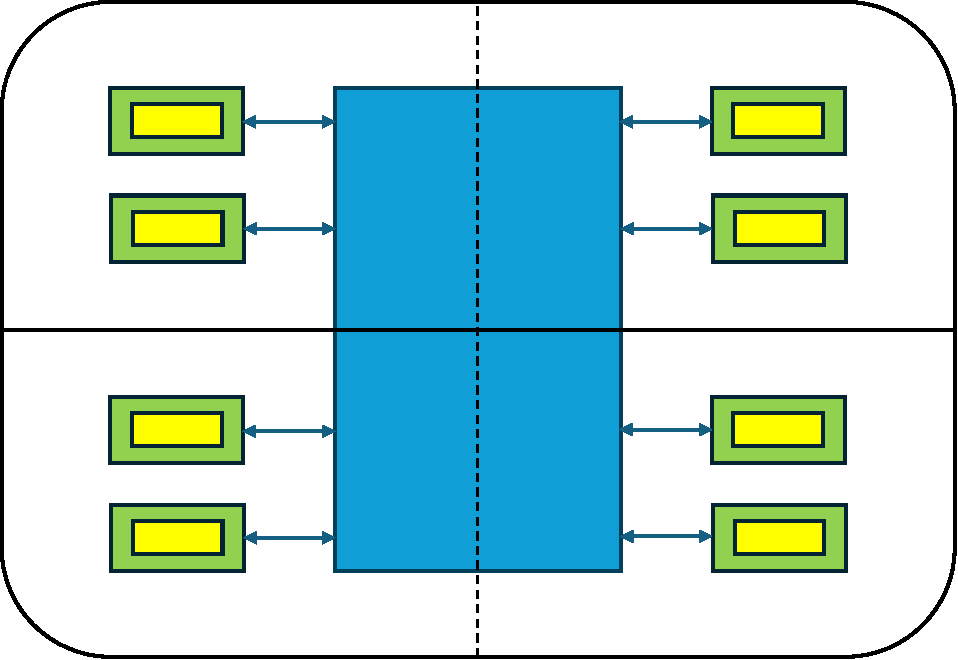
\includegraphics[width=0.56\textwidth]{figure/FIG_Topology_9242.pdf}};     /// overleaf
      \begin{scope}[x={(image.south east)},y={(image.north west)}]
          % \draw[help lines, step=1em] (-1em,-1em) grid (30em,20em);    
          % % Draw axes
          % \draw[dashed,->] (-1em,0) -- (30em,0) node[right] {x};
          % \draw[dashed,->] (0,-1em) -- (0,20em) node[above] {y};
  
        \node at (12em,18em) {$2$ $Scokets$};
  
        \node at (4.5em,1em) {$DDR4$};
        \node at (19.5em,1em) {$DDR4$};
  
        \node at (4.5em, 15em) {$DDR4$};
        \node at (19.5em,15em) {$DDR4$};
  
        \node at (12em,13em) {Hyper-threads};
        \node at (12em,5.5em) {Hyper-threads};
  
        \node at (12em,11em) {$48$ $CPUS$};
        \node at (12em,3.5em) {$48$ $CPUS$};
      \end{scope}
    \end{tikzpicture}
    \caption{NUMA topology of single node on Cluster}
    \label{FIG_Topology_Callan}
  \end{figure}



\end{frame}


\begin{frame}
  \frametitle{Single Node Scaling Tests}
  \framesubtitle{Strong Scaling - pure MPI}
  \begin{figure}[htbp]
    \centering
    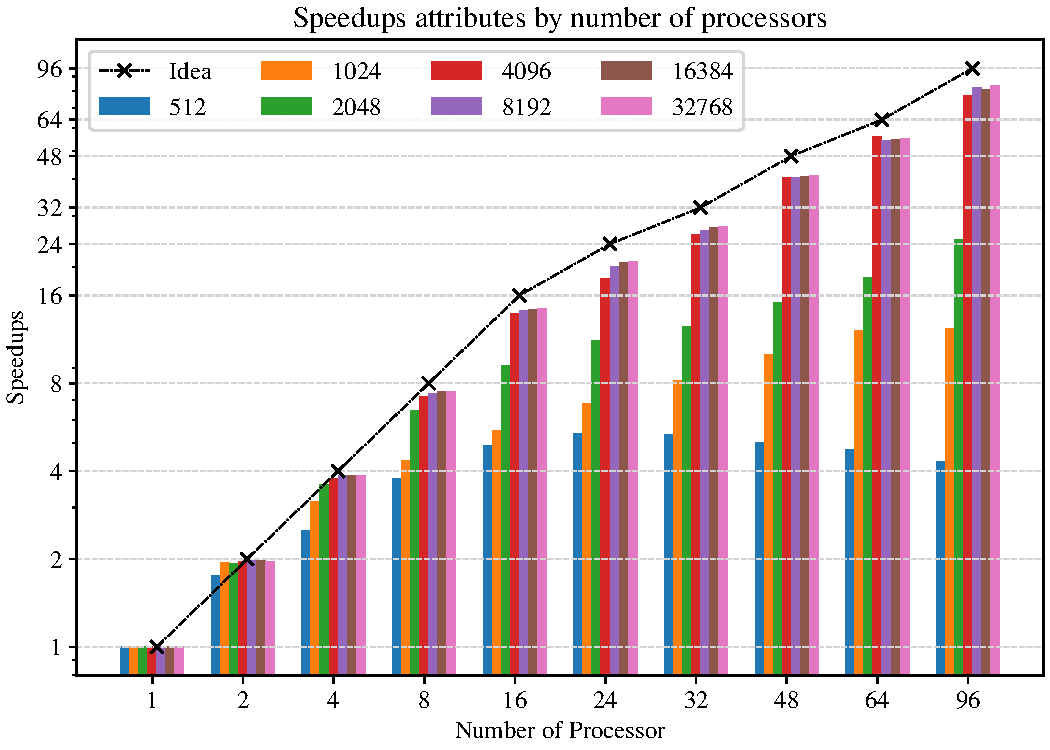
\includegraphics[width=0.56\textwidth]{figure/FIG_Benchmark_pure_mpi.pdf}
    \label{FIG:Benchmark:PURE_MPI}
  \end{figure}
\end{frame}



\begin{frame}
  \frametitle{Single Node Scaling Tests}
  \framesubtitle{Strong Scaling - MPI/OpenMP Hybrid}
  \begin{figure}
    \centering
    \begin{subfigure}{0.41\textwidth}
      \centering
      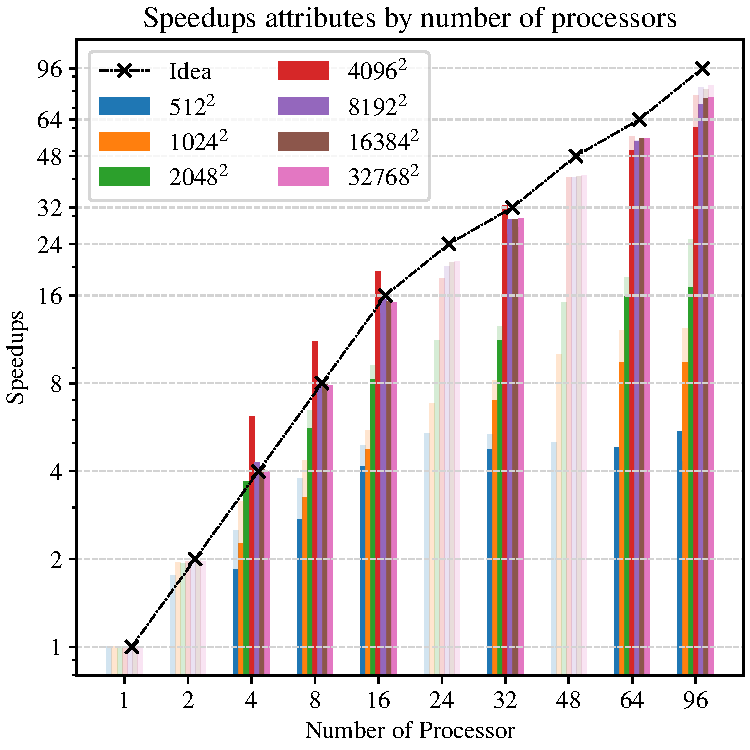
\includegraphics[width=\textwidth]{figure/FIG_Benchmark_hybrid_0.pdf}
      \caption{No overlapping comm./comp.}
      \label{FIG:Benchmark:Hybrid_0}
    \end{subfigure}
    % \hfill
    \begin{subfigure}{0.41\textwidth}
      \centering
      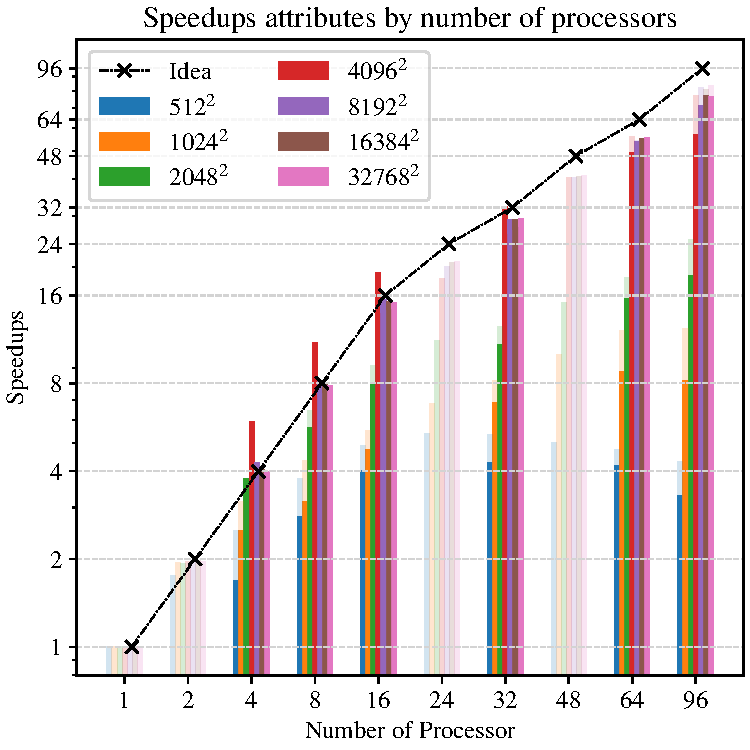
\includegraphics[width=\textwidth]{figure/FIG_Benchmark_hybrid_1.pdf}
      \caption{With overlapping comm./comp.}
      \label{FIG:Benchmark:Hybrid_1}
    \end{subfigure}
    % \caption{
    %   Comparison of speedup ratios of strong scaling tests of master-only parallelized program with overlapping and no overlapping of computation and communication.  
    %   The vague background is the results of pure MPI parallelization from Figure \ref{FIG:Benchmark:PURE_MPI}, and the problem scales are identical as well.
    %   The number of threads are set to $1$, $2$, $4$, $8$, $16$, and $24$, 
    %   tasks per CPU are $1$, $2$ and $4$.
    % }
    \label{FIG:Benchmark:Hybrid}
  \end{figure}
\end{frame}

\begin{frame}
  \frametitle{Single Node Scaling Tests}
  \framesubtitle{Weak Scaling}

  \begin{center}
    % \captionof{table}{Weak Scaling on Single Node of 2D Heat Equation}  % Use captionof to replace table environment
    \label{TAB:Benchmark:Weak_PURE_MPI}
    \footnotesize
    \begin{tabular}{p{3cm} p{1.5cm} p{1.5cm} p{1.5cm} p{1.5cm} p{1cm}}
      \toprule
      \multirow{2}{*}{\bfseries Strategy}     & \multirow{2}{*}{\bfseries Size} & \multicolumn{3}{c}{\bfseries Number of CPUs}   & \multirow{2}{*}{\bfseries $f_p(\%)$}  \\
                                    &                                  & \bfseries 4   & \bfseries 16   & \bfseries 64  &                                       \\
      \midrule
      \bfseries Pure MPI      & \multirow{3}{*}{$512^2$}      & 4.006  & 12.497  & 47.849                                         & 75.1 \\
      \bfseries No Overlap    &                               & 2.876  & 11.206  & 42.754                                         & 67.0 \\
      \bfseries With Overlap  &                               & 3.173  & 10.818  & 42.282                                         & 66.2 \\
      \midrule
      \bfseries Pure MPI      & \multirow{3}{*}{$1024^2$}     & 3.838  & 9.304   & 33.707                                         & 53.2  \\
      \bfseries No Overlap    &                               & 3.947  & 12.995  & 33.447                                         & 54.1 \\
      \bfseries With Overlap  &                               & 4.024  & 12.932  & 33.361                                         &  54.0 \\
      \midrule
      \bfseries Pure MPI      & \multirow{3}{*}{$2048^2$}     & 2.376  & 8.245   & 31.203                                         &  49.0\\
      \bfseries No Overlap    &                               & 3.874  & 8.972   & 31.510                                         &  49.8 \\
      \bfseries With Overlap  &                               & 3.740  & 8.989   & 31.430                                         &  49.7 \\
      \midrule
      \bfseries Pure MPI      & \multirow{3}{*}{$4096^2$}     & 3.543  & 8.245   & 31.203                                         &  77.5\\
      \bfseries No Overlap    &                               & 3.953  & 13.799  & 49.515                                         &  78.0\\
      \bfseries With Overlap  &                               & 3.948  & 13.800  & 49.989                                         &  78.7 \\
      \bottomrule
    \end{tabular}
  \end{center}
\end{frame}






\subsection{On Multi-node}
\begin{frame}
  \frametitle{Multi-node Scaling Tests}
  \framesubtitle{Strong Scaling - pure MPI}

  \begin{figure}[htbp]
    \centering
    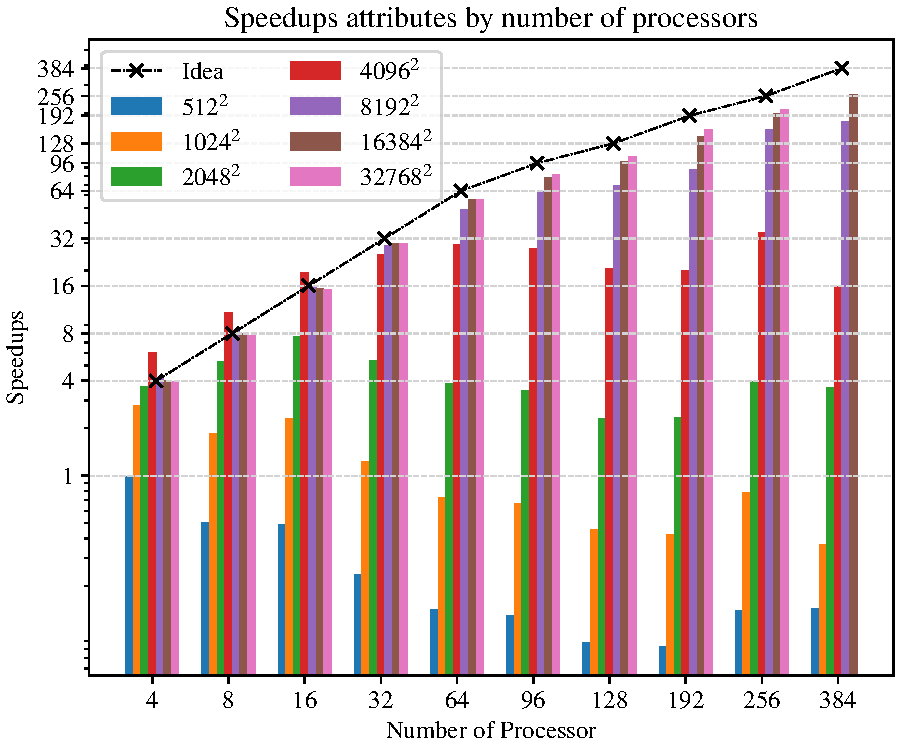
\includegraphics[width=0.55\textwidth]{figure/FIG_Benchmark_pure_mpi_multi_nodes.pdf}
    \caption{
      Comparison of speedup ratios of strong scaling tests of pure MPI parallelized program. 
      The investigated problem scales are the power of $2$, exponents ranging from $9$ to $15$.
      The number of CPUs are also set as power of $2$, with additional numbers $96$, $192$ and $384$ matched the topologies of CPU.
    }
    \label{FIG:Benchmark:PURE_MPI_Multi_Node}
  \end{figure}
\end{frame}



\begin{frame}
  \frametitle{Single Node Scaling Tests}
  \framesubtitle{Strong Scaling - MPI/OpenMP Hybrid}
  \begin{figure}
    \centering
    \begin{subfigure}{0.47\textwidth}
      \centering
      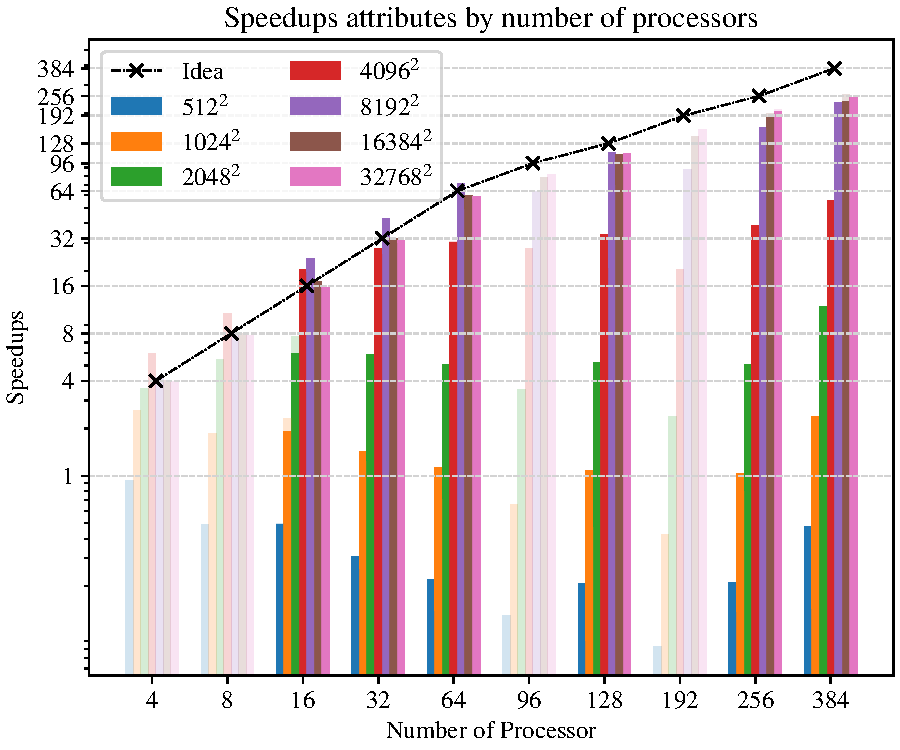
\includegraphics[width=\textwidth]{figure/FIG_Benchmark_hybrid_0_multi_nodes.pdf}
      \caption{No overlapping comm./comp.}
      \label{FIG:Benchmark:Hybrid_0_Multi_Node}
    \end{subfigure}
    % \hfill
    \begin{subfigure}{0.47\textwidth}
      \centering
      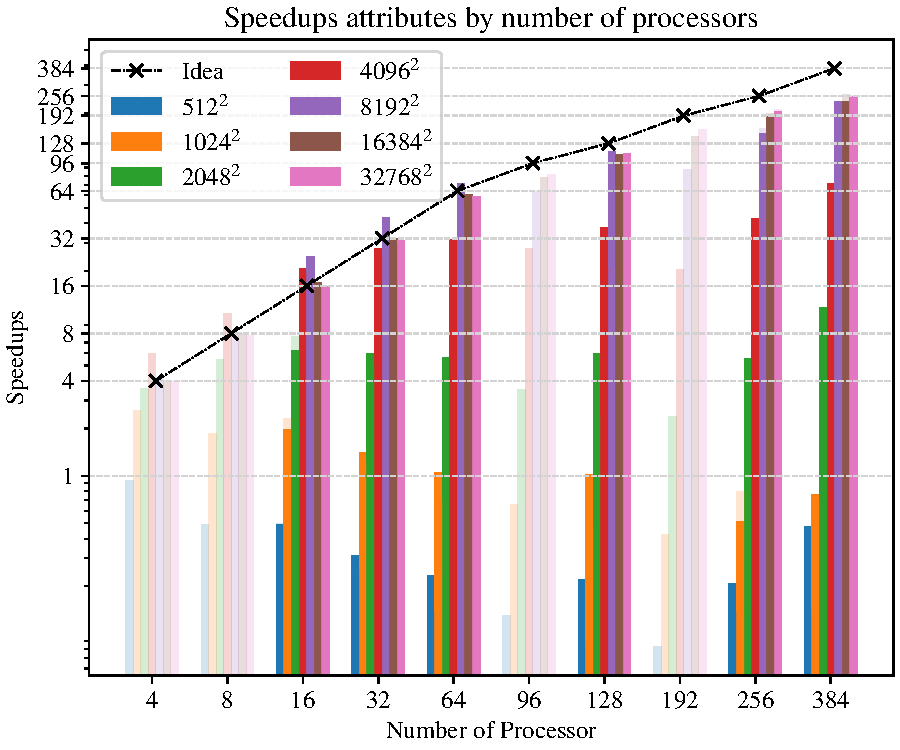
\includegraphics[width=\textwidth]{figure/FIG_Benchmark_hybrid_1_multi_nodes.pdf}
      \caption{With overlapping comm./comp.}
      \label{FIG:Benchmark:Hybrid_1_Multi_Node}
    \end{subfigure}
    % \caption{
      % Comparison of speedup ratios of strong scaling tests on $4$ nodes of 
      % mater-only parallelized program with overlapping and no overlapping of computation and communication.  
      % The vague background is the results of pure MPI parallelization from figure 
      % \ref{FIG:Benchmark:PURE_MPI_Multi_Node} and problems sclaes are identical as well.
      % The number of threads are set to $1$, $2$, $4$, $8$, $16$, and $24$, 
      % tasks per CPU are $1$, $2$ and $4$.
    % }
    \label{FIG:Benchmark:Hybrid_Multi_Node}
  \end{figure}
\end{frame}


\begin{frame}
  \frametitle{Single Node Scaling Tests}
  \framesubtitle{Weak Scaling}

  % \begin{table}[htbp]
  %   \caption{Weak Scaling on Multi-node of 2D Heat Equation}
  %   \label{TAB:Benchmark:Weak_PURE_MPI_Multi_Node}
  %   \begin{minipage}{\columnwidth}
  %     \begin{center}
  %       \footnotesize % overleaf
  %       \begin{tabular}{>{\bfseries}p{3cm} p{1.5cm} p{1.5cm} p{1.5cm} p{1.5cm} p{1.5cm} p{1cm}}
  %         \toprule
  %         \multirow{2}{*}{Strategy}     & \multirow{2}{*}{\bfseries Size} & \multicolumn{4}{c}{\bfseries  Number of CPUs}   & \multirow{2}{*}{\bfseries $f_p(\%)$}  \\
  %                                       &                                 & \bfseries 4   & \bfseries 16   & \bfseries 64  & \bfseries 256  &                        \\
  %         \midrule
  %         Pure MPI      & \multirow{3}{*}{$512^2$}      & 3.300  & 10.379  & 26.000   & 124.375                                    & 48.2 \\
  %         No Overlap    &                               &   -    &  8.094  & 25.931   & 127.648                                    & 49.3 \\
  %         With Overlap  &                               &   -    &  8.386  & 27.126   & 116.951                                    & 45.5 \\
  %         \midrule
  %         Pure MPI      & \multirow{3}{*}{$1024^2$}     & 3.848  & 13.037  & 30.143   &   -                                        & 49.3 \\
  %         No Overlap    &                               &   -    & 13.702  & 44.040   &   -                                        & 69.8 \\
  %         With Overlap  &                               &   -    & 13.834  & 44.090   &   -                                        & 69.9 \\
  %         \midrule
  %         Pure MPI      & \multirow{3}{*}{$2048^2$}     & 3.787  & 9.172   & 32.013   &   -                                        & 50.6 \\
  %         No Overlap    &                               &   -    & 13.936  & 34.368   &   -                                        & 55.7 \\
  %         With Overlap  &                               &   -    & 14.274  & 34.414   &   -                                        & 55.9 \\
  %         \midrule
  %         Pure MPI      & \multirow{3}{*}{$4096^2$}     & 3.884  & 13.859  & 51.041   &   -                                        & 80.2 \\
  %         No Overlap    &                               &   -    & 15.315  & 53.157   &   -                                        & 83.8 \\
  %         With Overlap  &                               &   -    & 15.294  & 53.401   &   -                                        & 84.2 \\
  %         \bottomrule
  %       \end{tabular}
  %     \end{center}
  %     % \bigskip
  %     % \footnotesize\emph{Source:} This is source 
  %   \end{minipage}
  % \end{table}


  \begin{center}
    % \caption{Weak Scaling on Multi-node of 2D Heat Equation}  % Use captionof to replace table environment
    \label{TAB:Benchmark:Weak_PURE_MPI_Multi_Node}
    \footnotesize
    \begin{tabular}{p{3cm} p{1.5cm} p{1.5cm} p{1.5cm} p{1.5cm} p{1.5cm} p{1cm}}
      \toprule
      \multirow{2}{*}{\bfseries Strategy}     & \multirow{2}{*}{\bfseries Size} & \multicolumn{4}{c}{\bfseries  Number of CPUs}   & \multirow{2}{*}{\bfseries $f_p(\%)$}  \\
                                    &                                 & \bfseries 4   & \bfseries 16   & \bfseries 64  & \bfseries 256  &                        \\
      \midrule
      \bfseries Pure MPI      & \multirow{3}{*}{$512^2$}      & 3.300  & 10.379  & 26.000   & 124.375                                    & 48.2 \\
      \bfseries No Overlap    &                               &   -    &  8.094  & 25.931   & 127.648                                    & 49.3 \\
      \bfseries With Overlap  &                               &   -    &  8.386  & 27.126   & 116.951                                    & 45.5 \\
      \midrule
      \bfseries Pure MPI      & \multirow{3}{*}{$1024^2$}     & 3.848  & 13.037  & 30.143   &   -                                        & 49.3 \\
      \bfseries No Overlap    &                               &   -    & 13.702  & 44.040   &   -                                        & 69.8 \\
      \bfseries With Overlap  &                               &   -    & 13.834  & 44.090   &   -                                        & 69.9 \\
      \midrule
      \bfseries Pure MPI      & \multirow{3}{*}{$2048^2$}     & 3.787  & 9.172   & 32.013   &   -                                        & 50.6 \\
      \bfseries No Overlap    &                               &   -    & 13.936  & 34.368   &   -                                        & 55.7 \\
      \bfseries With Overlap  &                               &   -    & 14.274  & 34.414   &   -                                        & 55.9 \\
      \midrule
      \bfseries Pure MPI      & \multirow{3}{*}{$4096^2$}     & 3.884  & 13.859  & 51.041   &   -                                        & 80.2 \\
      \bfseries No Overlap    &                               &   -    & 15.315  & 53.157   &   -                                        & 83.8 \\
      \bfseries With Overlap  &                               &   -    & 15.294  & 53.401   &   -                                        & 84.2 \\
      \bottomrule
    \end{tabular}
  \end{center}
\end{frame}


\subsection{On Different Dimensions}
\begin{frame}
  \frametitle{3D Space Heat Equation}
  \framesubtitle{Strong Scaling - pure MPI}
  
  \begin{figure}
    \centering
    \begin{subfigure}{0.42\textwidth}
      \centering
      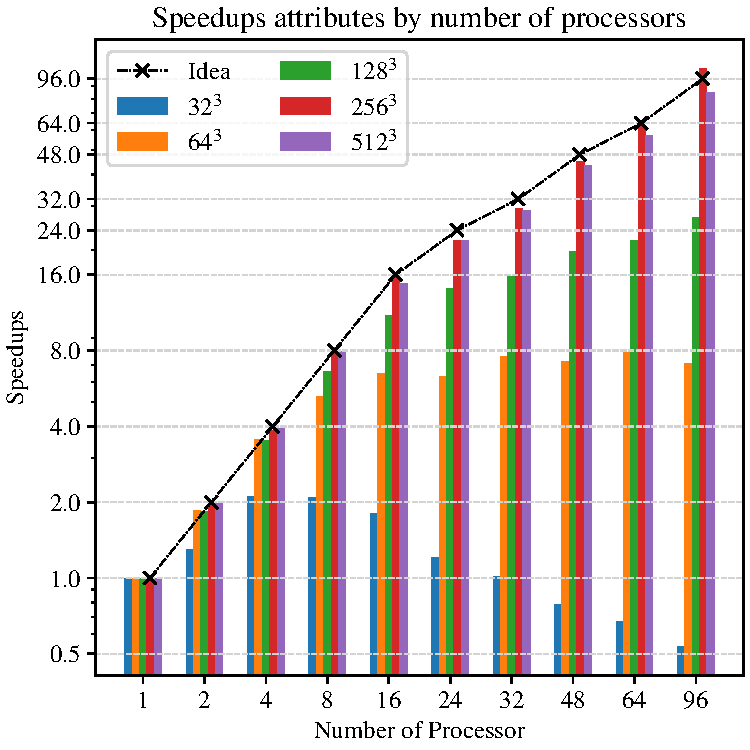
\includegraphics[width=\textwidth]{figure/FIG_Benchmark_pure_mpi_3D.pdf}
      \caption{Single node}
      \label{FIG:Benchmark:Pure_MPI_Single_Node_3D}
    \end{subfigure}
    % \hfill
    \begin{subfigure}{0.42\textwidth}
      \centering
      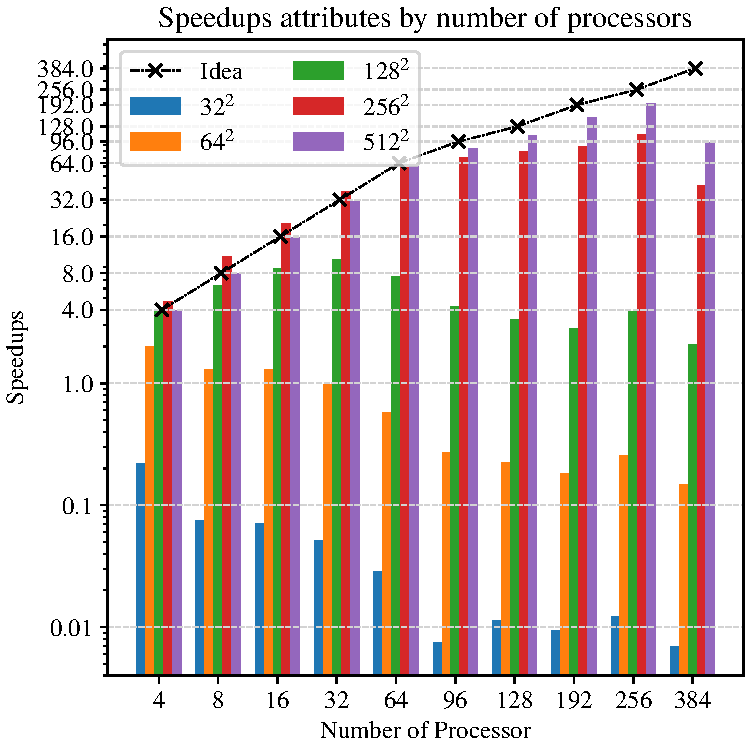
\includegraphics[width=\textwidth]{figure/FIG_Benchmark_pure_mpi_3D_multi_nodes.pdf}
      \caption{Four nodes}
      \label{FIG:Benchmark:Pure_MPI_Multi_Node_3D}
    \end{subfigure}
    % \caption{
      % Comparison of speedup ratios of strong scaling tests  pure MPI models on $4$ nodes of and $1$ node.
      % The problem sizes are set to $32^3$, $64^3$, $128^3$, $256^3$ and $512^3$ with single precision.
    % }
    \label{FIG:Benchmark:Pure_MPI_Node_3D}
  \end{figure}
  
\end{frame}



\begin{frame}
  \frametitle{3D Space Heat Equation}
  \framesubtitle{Strong Scaling - MPI/OpenMP Hybrid, Single Node}



  \begin{figure}
    \centering
    \begin{subfigure}{0.42\textwidth}
      \centering
      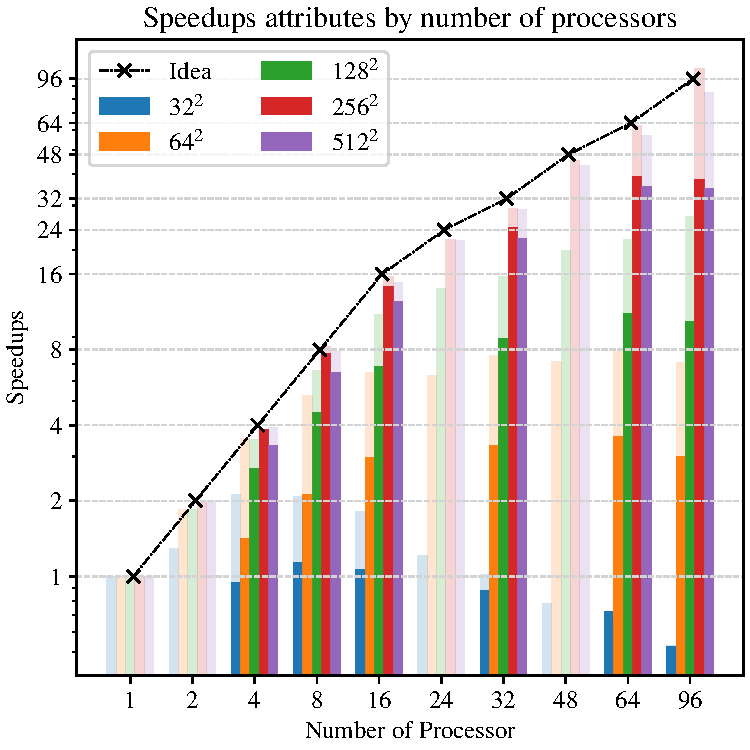
\includegraphics[width=\textwidth]{figure/FIG_Benchmark_hybrid_0_single_nodes_3D.pdf}
      \caption{Non-overlapping}
      \label{FIG:Benchmark:FIG_Benchmark_hybrid_0_single_nodes_3D}      
    \end{subfigure}
    % \hfill
    \begin{subfigure}{0.42\textwidth}
      \centering
      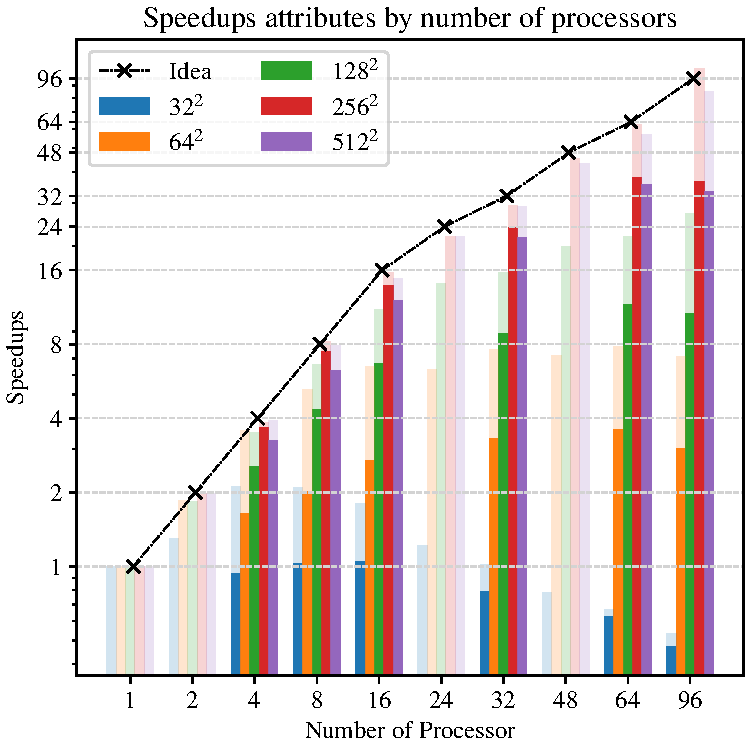
\includegraphics[width=\textwidth]{figure/FIG_Benchmark_hybrid_1_single_nodes_3D.pdf}
      \caption{With overlapping}
      \label{FIG:Benchmark:FIG_Benchmark_hybrid_1_single_nodes_3D}
    \end{subfigure}
    % \caption{
      % Comparison of speedup ratios of strong scaling tests  pure MPI models on $4$ nodes of and $1$ node.
      % The problem sizes are set to $32^3$, $64^3$, $128^3$, $256^3$ and $512^3$ with single precision.
    % }
    \label{FIG:Benchmark:Hybrid_Single_Node_3D}
  \end{figure}

\end{frame}






% \begin{figure}[htbp]
%   \centering
%   \subfigure[Single Node, Non-overlapping]{
%     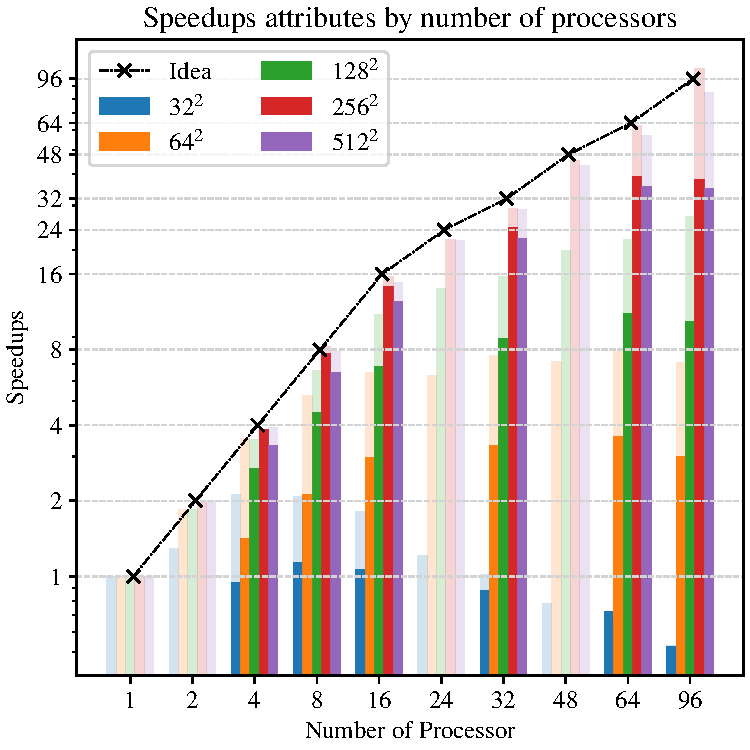
\includegraphics[width=0.38\textwidth]{figure/FIG_Benchmark_hybrid_0_single_nodes_3D.pdf}
%     \label{FIG:Benchmark:FIG_Benchmark_hybrid_0_single_nodes_3D}
%   }
%   \hspace{0em} 
%   \subfigure[Single Node, With overlapping]{
%     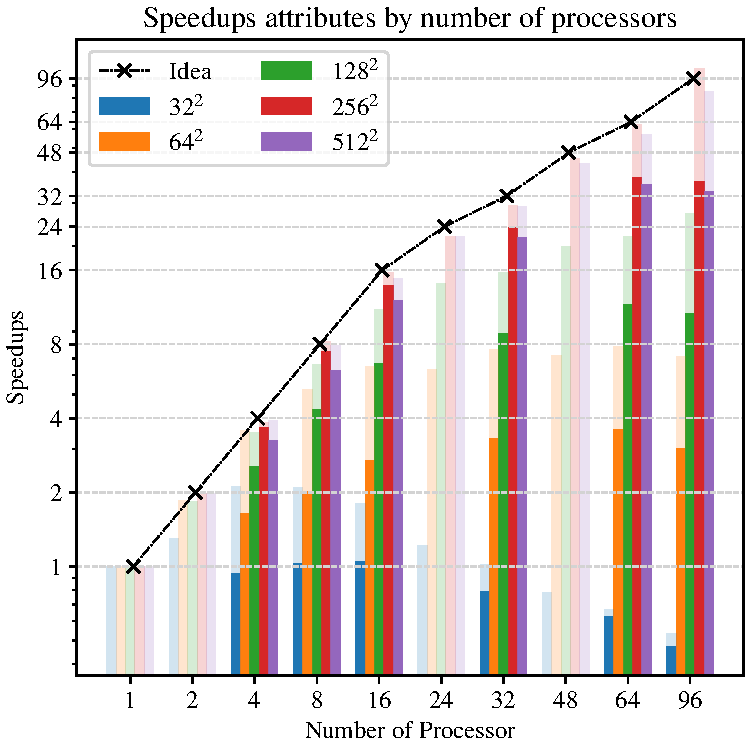
\includegraphics[width=0.38\textwidth]{figure/FIG_Benchmark_hybrid_1_single_nodes_3D.pdf}
%     \label{FIG:Benchmark:FIG_Benchmark_hybrid_1_single_nodes_3D}
%   }
%   \hspace{0em} 
%   \subfigure[Multi-node, Non-overlapping]{
%     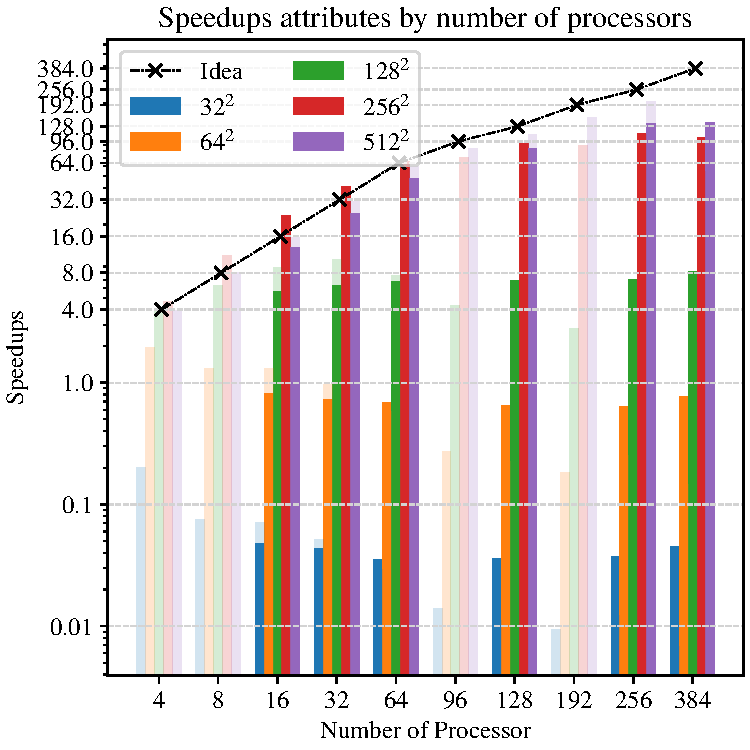
\includegraphics[width=0.38\textwidth]{figure/FIG_Benchmark_hybrid_0_multi_nodes_3D.pdf}
%     \label{FIG:Benchmark:FIG_Benchmark_hybrid_0_multi_nodes_3D}
%   }
%   \hspace{0em} 
%   \subfigure[Multi-node, With overlapping]{
%     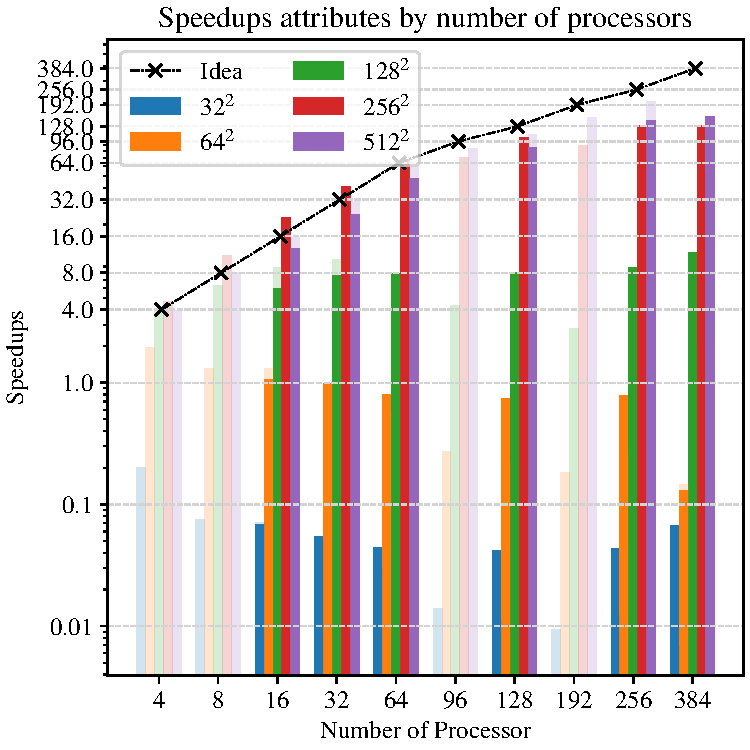
\includegraphics[width=0.38\textwidth]{figure/FIG_Benchmark_hybrid_1_multi_nodes_3D.pdf}
%     \label{FIG:Benchmark:FIG_Benchmark_hybrid_1_multi_nodes_3D}
%   }
%   \caption{
%       Comparison of strong scaling speedup ratios of hybrid models on $4$ compute nodes for solving 3D heat euqations.
%       The problem scales are set to the cude of $32$, $64$, $128$, $256$ and $512$ with single precision.
%       The value background is the strong scaling results of figure \ref{FIG:Benchmark:Pure_MPI_Node_3D}.
%     }
%   \label{FIG:Benchmark:Hybrid_Single_Four_Node_3D}
% \end{figure}



\begin{frame}
  \frametitle{3D Space Heat Equation}
  \framesubtitle{Strong Scaling - MPI/OpenMP Hybrid, Four Nodes}
  

  
  \begin{figure}
    \centering
    \begin{subfigure}{0.42\textwidth}
      \centering
      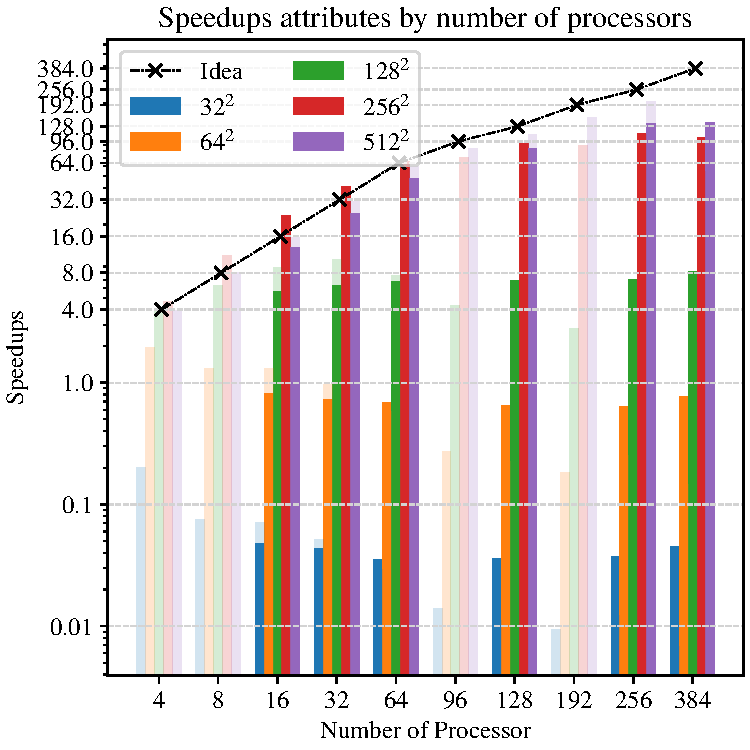
\includegraphics[width=\textwidth]{figure/FIG_Benchmark_hybrid_0_multi_nodes_3D.pdf}
      \caption{Non-overlapping}
      \label{FIG:Benchmark:FIG_Benchmark_hybrid_0_multi_nodes_3D}
    \end{subfigure}
    % \hfill
    \begin{subfigure}{0.42\textwidth}
      \centering
      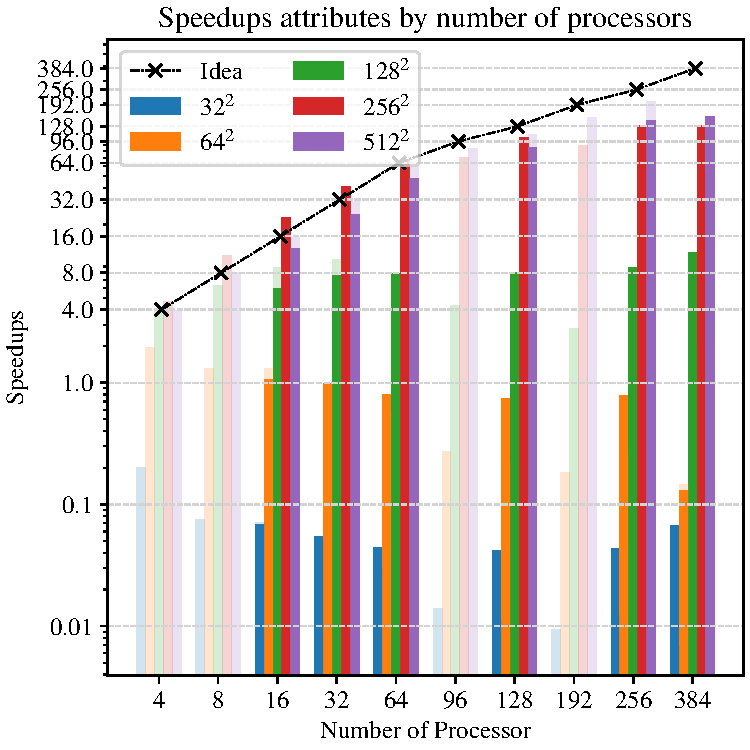
\includegraphics[width=\textwidth]{figure/FIG_Benchmark_hybrid_1_multi_nodes_3D.pdf}
      \caption{With overlapping}
      \label{FIG:Benchmark:FIG_Benchmark_hybrid_1_multi_nodes_3D}
    \end{subfigure}
    % \caption{
      % Comparison of speedup ratios of strong scaling tests  pure MPI models on $4$ nodes of and $1$ node.
      % The problem sizes are set to $32^3$, $64^3$, $128^3$, $256^3$ and $512^3$ with single precision.
    % }
    \label{FIG:Benchmark:Hybrid_Four_Node_3D}
  \end{figure}

  
\end{frame}



\begin{frame}
  \frametitle{3D Space Heat Equation}
  \framesubtitle{Weak Scaling}


  % \begin{table}[htbp]
    % \caption{Weak Scaling of 3D Heat Equation}
  %   \label{TAB:Benchmark:Weak_3D_AllModels}
  %   \begin{minipage}{\columnwidth}
      \begin{center}
        \footnotesize % overleaf
        \begin{tabular}{p{2.5cm} p{1cm} p{1.5cm} p{1.5cm} p{1.5cm} p{1.5cm} p{1cm} p{1cm}}
          \toprule
          \multirow{2}{*}{\bfseries Strategy} & \multirow{2}{*}{\bfseries Size} & \multicolumn{3}{c}{\bfseries  Number of CPUs}    & \multirow{2}{*}{\bfseries $f_p(\%)$}  & \multirow{2}{*}{\bfseries $f_p(\%)_{\text{Multi-node}}$}\\
                        &                      & \bfseries 8     & \bfseries 64        & \bfseries 64$_{\text{Multi-node}}$   &  &  &         \\
          \midrule
          \bfseries Pure MPI      & \multirow{3}{*}{$32^3$}       & 5.243  & 26.405              &  9.078                     & 41.6 & 14.2 \\
          \bfseries No Overlap    &                               & 2.124  & 13.386              &  8.094                     & 21.0 &  12.7\\
          \bfseries With Overlap  &                               & 2.014  & 13.884              &  9.586                     & 21.8 & 39.7 \\
          \midrule
          \bfseries Pure MPI      & \multirow{3}{*}{$64^3$}       & 7.937  & 32.034              &  30.106                    & 50.8 & 47.1 \\
          \bfseries No Overlap    &                               & 5.393  & 20.007              &  33.460                    & 31.8 & 52.3 \\
          \bfseries With Overlap  &                               & 5.200  & 19.558              &  35.254                    & 31.1 & 31.6 \\
          \midrule
          \bfseries Pure MPI      & \multirow{3}{*}{$128^3$}      & 3.513  & 24.239              &  25.428                    & 38.0 & 39.7 \\
          \bfseries No Overlap    &                               & 3.303  & 15.235              &  35.254                    & 24.1 & 55.1 \\
          \bfseries With Overlap  &                               & 3.187  & 15.107              &  20.096                    & 23.9 & 31.4 \\
          \bottomrule
        \end{tabular}
      \end{center}
      % \bigskip
      % \footnotesize\emph{Source:} This is source 
  %   \end{minipage}
  % \end{table}
  

\end{frame}






\subsection{With PINN on accuracy}


\begin{frame}
  \frametitle{PINN v.s. FDTD}
  \framesubtitle{Accuracy}

  \begin{table}
    \caption{Mean Square Error of Results}
    \begin{center}
      \footnotesize
      \begin{tabular}{p{1.5cm} p{1.5cm} p{1.5cm}}
        \toprule
        \bfseries Method  & \bfseries Heat 2D      & \bfseries Heat 3D         \\
        \midrule 
        \bfseries FDTD    & 1.7287  & 953.84 \\
        \bfseries PINN    & 13.37   & 24.896 \\
        \bottomrule 
        \multicolumn{3}{l}{Tolerance: $10^{-4}$} \\
      \end{tabular}
    \end{center}
  \end{table}


  

\end{frame}

\begin{frame}
  \frametitle{PINN v.s. FDTD}
  \framesubtitle{Memory Usage v.s. Time of Convergence}

  
  \begin{figure}[htbp]
    \centering
    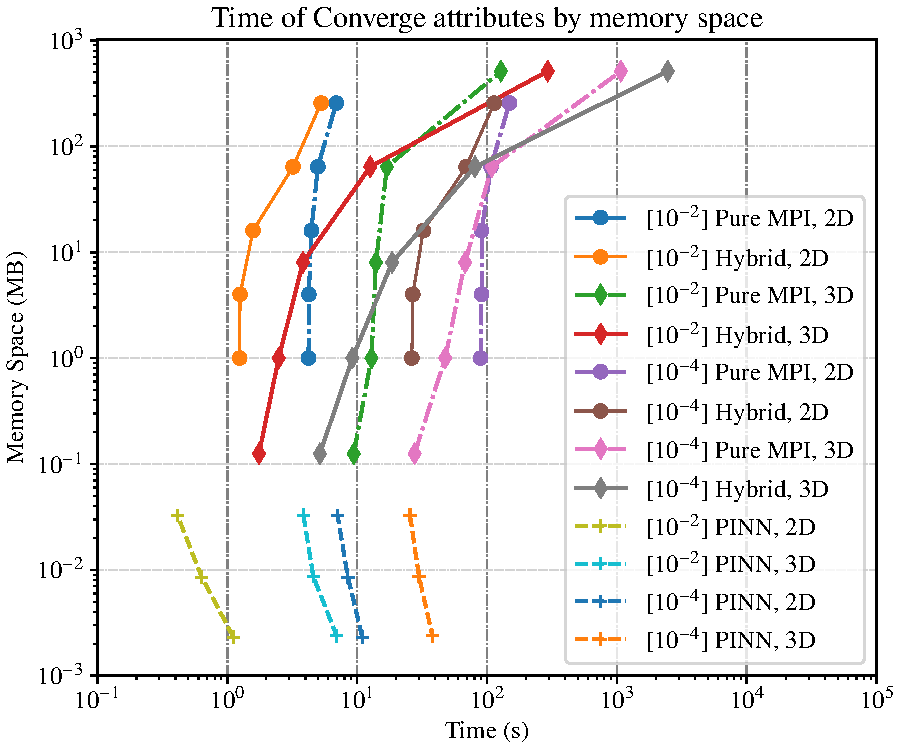
\includegraphics[width=0.45\textwidth]{figure/FIG_Benchmark_Time_Tol.pdf}
    \caption{
      % Comparison of memory usage of FDTD and PINN attributed by time of trainning/converging time consumption for 
      % both 2 dimension and 3 dimension heat equations with single precision. 
      % The predefined tolerance for training and converging are $10^{-2}$ and $10^{-4}$.
      % FDTD was testing on four compute nodes (384 CPUs), and using pure MPI and non-overlapping hybrid models.
      % The PINN models are trained on single NVIDIA RTX 4090 graphics card.
    }
    \label{FIG:Benchmark:TimeTol}
  \end{figure}
\end{frame}


\section{Discussion}
% \subsection{Conclusion}
\begin{frame}
  \frametitle{}

  

\end{frame}



% \subsection{Further Work}
% \begin{frame}
%   \frametitle{}

  

% \end{frame}



\begin{frame}
  \frametitle{Closing Remarks}
  \centering
  {\Large Thank you for your attention!}\\
  \vspace{2em}
  {\large Any questions?}
\end{frame}


% \begin{frame}[allowframebreaks]
%   \frametitle{References}
%   \printbibliography
% \end{frame}

\end{document}

